% TODO:
% - Make a tool for download and transformation of datasets, and sell the work that I have done
% - Compare single user datasets
% - group rec datasets mention
% - do dataset group augmentation and add it to the tool


\chapter{Datasets}  \label{chap:datasets}
People are gregarious in nature, but the same, unfortunately, cannot be said about machine learning datasets. Vast majority of them are not directly usable in the group RS research due to only containing information about single user preference. In order to design and evaluate group recommender systems, we preferably need datasets that contain information about groups' preference.

In this chapter, we will start with description of which datasets are suitable for the use in RS domain. We describe commonly used datasets in the non-group RS domain. Analyse their high level properties and describe what transformations are needed in order to make the use of the dataset convenient. 

Next, we will talk about the existing group RS datasets and introduce methods that can be used to generate the group recommendation information synthetically from non-group RS datasets. We will use these methods to generate standardized synthetically enriched group RS datasets from non-group datasets that we will describe in the single user datasets subchapter.

And finally, we describe a data transformation library that we create for the purpose of simplifying the research efforts in the RS domain and for evaluation of our proposed algorithm.

% We will first describe a few of the popular datasets which we have determined to be used as research data the most. Then we will 

% -------------------------------------------------------------------------------------
\section{Single user datasets} \label{sec:single_user_datasets}
% -------------------------------------------------------------------------------------
Multiple well known and thoroughly studied datasets exist in the recommender system domain. Let us now present the popular ones that seems to be utilized the most.

If we talk about specific format of the data then we are referring to the unified format which we have transformed the original data into using the dataset transformation library. Further description about the data format transformations follow in \ref{subsec:04_single_user_datasets.gathering_processing}.



% -------------------------------------------------------------------------------------
\subsection{Movie Lens}
% -------------------------------------------------------------------------------------
One of the most well known dataset in the RS domain, it contains 25 million ratings in total across 62,000 movies and 162,000 users. The data were collected between 1995 and 2019 and the current version of this size (25M) was released in November of 2019. Data are organic and come from a web-based recommendation system at \href{https://movielens.org/}{movielens.org}. The project was specifically created in order to gather research data on personalized recommendation by researches at University of Minnesota.

Dataset is in a good format that is quite easy to parse and use. Further description follows in \ref{subsec:04_single_user_datasets.gathering_processing}.

\hfill \break
\noindent
\textbf{Number of items:} 62,000 \newline
\textbf{Number of users:} 162,000 \newline
\textbf{Number of user-item interactions:} 25,000,095 \newline
\textbf{User-item interactions format:} Sparse matrix of ordinal ratings [1, 1.5, 2, ... 4.5, 5] - user rated a movie \newline
\textbf{List of datatables:} Movies (detail in Table \ref{table:5.1_ML_movies}), Ratings (detail in Table \ref{table:5.1_ML_ratings}), Tags, Links, Genres, Genome Scores, Genome Tags

\begin{table}[ht!]
\centering
\begin{tabular}{ l l }
\verb|item_id| & \verb|title| \\
    \hline
     1  &                   Toy Story (1995) \\
     2  &                     Jumanji (1995) \\
     3  &            Grumpier Old Men (1995) \\
   ...  &                                ... \\
209169  &                A Girl Thing (2001) \\
209171  &     Women of Devil's Island (1962) \\ [1mm]
\multicolumn{2}{l}{{[62423 rows x 2 columns]}}
\end{tabular}
\caption{Short snippet of Movie Lens dataset's \texttt{movies.csv} table.}
\label{table:5.1_ML_movies}
\end{table}

\begin{table}[!ht]
\centering
\begin{tabular}{ l l l l }

% \texttt{user\_id} & \texttt{item\_id} & \texttt{rating} & \texttt{timestamp} \\
\verb|user_id| & \verb|item_id| & \verb|rating| & \verb|timestamp| \\
    \hline
    1 &      296  &   5.0 & 1147880044 \\
    1 &      306  &   3.5 & 1147868817 \\
    1 &      307  &   5.0 & 1147868828 \\
  ... &      ...  &   ... &        ... \\
162541 &    58559  &   4.0 & 1240953434 \\
162541 &    63876  &   5.0 & 1240952515 \\ [1mm]
\multicolumn{4}{l}{{[25000095 rows x 4 columns]}}
\end{tabular}
\caption{Short snippet of Movie Lens dataset's \texttt{ratings.csv} table.}
\label{table:5.1_ML_ratings}
\end{table}

% This dateset contains information about movies in the form of \textit{'\textless movieId, title, genres\textgreater'}, ratings in the form of \textit{'\textless userId, movieId, rating, timestamp\textgreater'} and additional information about links, tags, genome-scores and genome-tags.




% -------------------------------------------------------------------------------------
\subsection{KGRec}
\label{subsec:04_single_user_datasets.kgrec}
% -------------------------------------------------------------------------------------
KGRec is a smaller and less known dataset. We have chosen this dataset because it was utilized in GFAR method introduced in \cite{GFAR-kaya2020} and described in \ref{subsec:03_advanced_methods.gfar}. This dataset consists of two separate datasets of music and sound, KGRec-music and KGRec-sound respectively.

The first music dataset comes from \href{https://www.songfacts.com/}{songfacts.com} (items and text descriptions) and \href{https://www.last.fm/}{last.fm} (ratings, items, tags). Each user-item interaction is a user listening to a song.

The second, sound dataset, comes from \href{https://freesound.org/}{freesound.org}. Items are sounds with description using text and tags that were created by the person that uploaded the sound. Each user-item interaction is a user downloading an item, in this case a sound.

Further, we will consider only the music dataset and not utilize the sound dataset at all. We have made this decision to simplify comparisons and due to the origin of the sound dataset itself. It comes from a web-page where users can upload and download random sounds of their choosing, such as 'Mechanical clock movement' sound, 'Industrial elevator' sound and so on. The need for these sounds are most probably driven from people that are using them for their profession, such as video production and therefore does not reflect natural content consumption preferences.

Both datasets were created for the needs of \cite{kgrec_dataset_origin}, where they were introduced, they are altered for the needs of research in Recommendation Knowledge Graphs. Further, the original data that were used for creation of this datasets are described in \cite{kgrec_dataset_origin_full}.


\hfill \break
\noindent
\textbf{Number of items:} 8,640; 21,552\footnote{Number of items, users and user-item interactions are in order - music dataset; sound dataset} \newline
\textbf{Number of users:} 5,199; 20,000 \newline
\textbf{Number of user-item interactions:} 751,531; 2,117,698 \newline
\textbf{User-item interactions format:} one-valued implicit feedback - user listened or downloaded a song/sound \newline
\textbf{List of datatables:} Ratings(detail in Table \ref{table:5.1_KGRec_ratings}), Tags, Descriptions

\begin{table}[!ht]
    \centering
    \begin{tabular}{ l l }
        \verb|user_id|   & \verb|item_id| \\
        \hline
        7596     &  68  \\
        7596     & 130  \\
        7596     & 330  \\
        ...      & ...  \\
        50572897 & 8618 \\
        50572897 & 8619 \\ [1mm]
        \multicolumn{2}{l}{{[751531 rows x 2 columns]}}
    \end{tabular}
    \caption{Short snippet of KGRec dataset's \texttt{music\_ratings.csv} table.}
    \label{table:5.1_KGRec_ratings}
\end{table}

% \newline
% Both dataset are in the form of '\textlessuser userId, itemId\textgreater'


% -------------------------------------------------------------------------------------
\subsection{Netflix Prize}
% -------------------------------------------------------------------------------------

Data that were originally released in 2009 by the Netflix.com video streaming company for the \textit{Netflix Prize}, open competition with main prize of 1 million dollars. It contains data of more than 400 thousand randomly selected users from the company's database. Data contain information about users ratings of movies. It was originally available on the contest web page, but has been removed since.

The original data was split into multiple files in a file for ratings per movie manner. Each rating is a quadruplet of the form '\textless user, movie, date of rating, rating\textgreater'.

\hfill \break
\noindent
\textbf{Number of items:} 17,770 \newline
\textbf{Number of users:} 480,189 \newline
\textbf{Number of user-item interactions:} 100,480,507 \newline
\textbf{User-item interactions format:} sparse matrix of ordinal ratings [1, 2, 3, 4, 5] \newline
\textbf{List of datatables:} Ratings (detail in Table \ref{table:5.1_Netflix_ratings}), Movies (detail in Table \ref{table:5.1_Netflix_movies})

\begin{table}[!ht]
    \centering
    \begin{tabular}{ l l l l }
        \verb|user_id| & \verb|item_id| & \verb|rating| & \verb|date| \\
        \hline
              6 &             30 &             3 &  2004-09-15 \\
              6 &            157 &             3 &  2004-09-15 \\
              6 &            173 &             4 &  2004-09-15 \\
            ... &            ... &           ... &         ... \\
        2649429 &          17627 &             3 &  2003-07-21 \\
        2649429 &          17692 &             2 &  2002-12-07 \\ [1mm]
        \multicolumn{4}{l}{{[100480507 rows x 4 columns]}}
    \end{tabular}
    \caption{Short snippet of Netflix dataset's \texttt{ratings.csv} table.}
    \label{table:5.1_Netflix_ratings}
\end{table}
    
\begin{table}[!ht]
    \centering
    \begin{tabular}{ l l l }
        \verb|item_id| & \verb|release_year| & \verb|title| \\
        \hline
            1 &       2003.0 &            Dinosaur Planet    \\
            2 &       2004.0 & Isle of Man TT 2004 Review    \\
            3 &       1997.0 &                  Character    \\
          ... &          ... &                        ...    \\
        17769 &       2003.0 &                The Company    \\
        17770 &       2003.0 &               Alien Hunter \\ [1mm]
        \multicolumn{3}{l}{{[17770 rows x 3 columns]}}
    \end{tabular}
    \caption{Short snippet of Netflix dataset's \texttt{movies.csv} table.}
    \label{table:5.1_Netflix_movies}
\end{table}
% -------------------------------------------------------------------------------------
\subsection{Spotify - Million Playlist Dataset}
% -------------------------------------------------------------------------------------
This dataset was released in January 2018 for \textit{The Spotify Milion Playlist Dataset Challenge}. It contains 1,000,000 playlists with information about tracks that are part of each playlist. Main purpose of this dataset was to study and develop better algorithms for automatic playlist continuation where the system would be able to recommend songs that are similar to those that are already in the playlist. In contrast to the Netflix challenge, no prize was to be awarded at the end of the challenge.

Even though the context of this dataset are playlists and not users, we utilize a different view on the dataset, where each playlist will represent a single user. This way, we have an another big and organic dataset at our disposal. It can therefore be used not only for playlist continuation tasks, but for the classical RS domain tasks as well. In a sense, a single playlist is a specific subset of preference of the user that have created the playlist. Therefore we expect to see a narrower preference distribution for each of these 'playlist' users.

For completeness, it is necessary to add that some playlists are 'collaborative', meaning that they were created by multiple users. But they account for only 2.3\% of all playlists, which in our opinion does not substantially affect the dataset. These collaborative datasets could be used as a group recommender dataset on their own, unfortunately, the information about which user added which track, to the collaborative playlist, is not present.

\begin{table}[!ht]
    \centering
    \begin{tabular}{ l l }
        \verb|playlist_id|   & \verb|item_id| \\
        \hline
        549000     &  0  \\
        549000     & 1  \\
        549000     & 2  \\
        ...      & ...  \\
        302999 & 133087 \\
        302999 & 133088 \\ [1mm]
        \multicolumn{2}{l}{{[66346428 rows x 2 columns]}}
    \end{tabular}
    \caption{Short snippet of Spotify Milion Playlist dataset's \texttt{ratings.csv} table.}
    \label{table:5.1_Spotify_ratings}
\end{table}


\begin{table}[!ht]
    \centering
    \begin{tabular}{ l l l }
        \verb|item_id| & \verb|item_name| & \verb|artist_name|  \\
        \hline
             0 & Boots of Spanish Leather &         Bob Dylan \\
             1 &       Mr. Tambourine Man &         Bob Dylan \\
             2 &             Danny's Song & Loggins \& Messina \\ 
           ... &                      ... &               ... \\
       2262290 &               Robin Hood &        Crazy Fool \\
       2262291 &                Guilttrip &      Ace Reporter \\ [1mm]
       \multicolumn{3}{l}{{[2262292 rows x 6 columns]}}
    \end{tabular}
    \caption[Short snippet of Netflix dataset's \texttt{tracks.csv} table.]{Short snippet of Netflix dataset's \texttt{tracks.csv} table. (Columns \texttt{item\_uri}, \texttt{artist\_uri}, \texttt{album\_uri}, containing URI to Spotify object were omitted for simplicity due to their substantial length.)}
    \label{table:5.1_Spotify_tracks}
\end{table}

\hfill \break
\noindent
\textbf{Number of items:} 2,262,292 \newline
\textbf{Number of users:} 1,000,000 \newline
\textbf{Number of user-item interactions:} 66,346,428 \newline
\textbf{User-item interactions format:} one-valued implicit feedback - user added a song to a playlist\newline
\textbf{List of datatables:} Tracks (detail in Table \ref{table:5.1_Spotify_tracks}), Ratings (detail in Table \ref{table:5.1_Spotify_ratings})




% -------------------------------------------------------------------------------------
\subsection{Comparison of datasets}
% -------------------------------------------------------------------------------------

\begin{figure}[ht!]
    \centering
    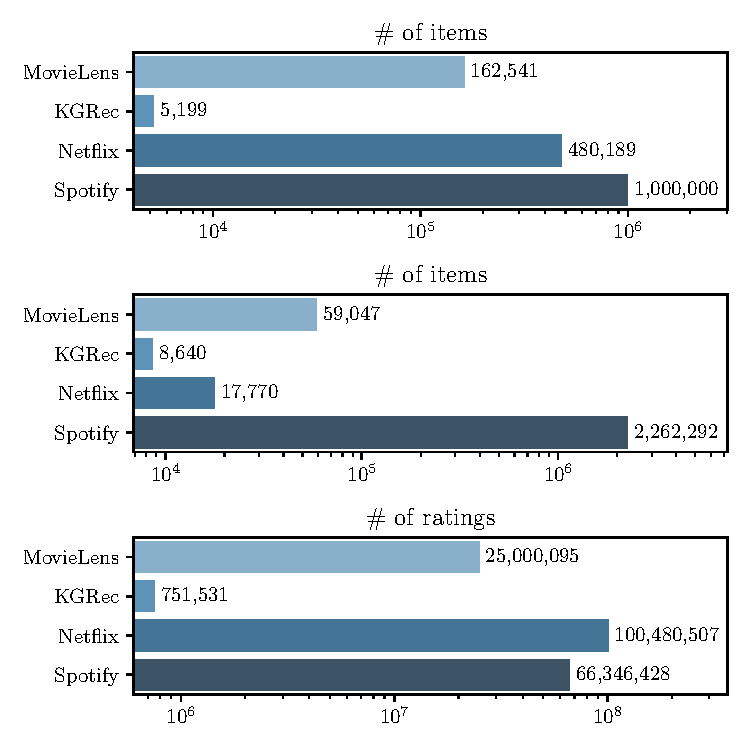
\includegraphics{img/figures/datasets_counts.pdf}
    \caption[Size comparison of the selected datasets.]{Size comparison of the selected datasets. All x-axes are log scale due to the big differences between the dataset.}
    \label{fig:datasets_counts}
\end{figure}

We have described each dataset separately, let us now compare them together to see how they differ. As we can see on Figure \ref{fig:datasets_counts} the Spotify and Netflix datasets are the biggest. We see that KGRec dataset is almost two orders of magnitude smaller than the rest of the datasets. As already mentioned, we have selected it due to it being utilized in the related literature. Spotify dataset is different by having two orders of magnitude more items, which can present a challenge on its own. If we for example use matrix factorization methods to compute the preference, then the amount of memory will rise by two orders of magnitude as well. Additionally, the sparsity of ratings is higher, which can negatively affect efficacy.

Movie Lens dataset has a potential benefit as it has actual ratings for each user-item interaction. All other presented datasets only contain user-item interactions in the form of one-valued implicit feedback.

\begin{figure}[ht!]
    \centering
    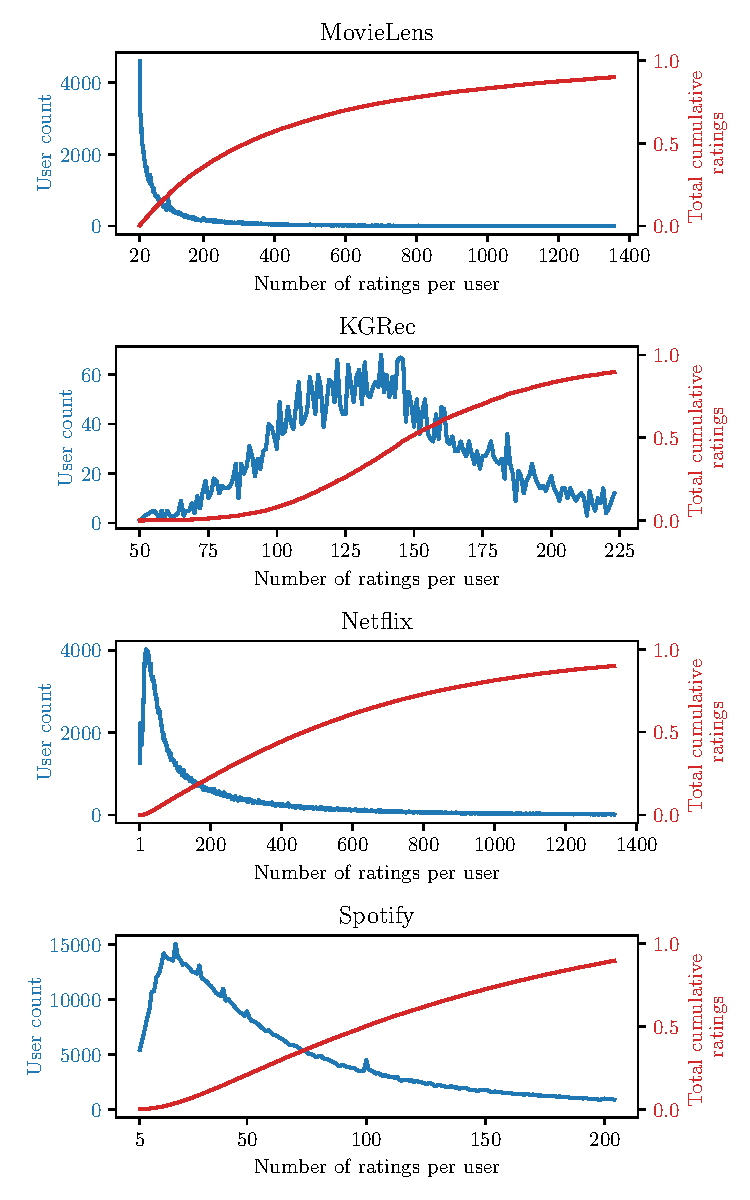
\includegraphics{img/figures/num_users_by_rating_count.pdf}
    \caption[Distribution of ratings]{Distribution of ratings for groups of users by how many ratings they have made. Blue line shows how many users have made that particular amount of ratings, while red line shows the total cumulative mass distribution of ratings. We have clipped the number of ratings by total cumulative ratings of 90\% due to very long-tailed data, where some small amount of users created a very high amount of ratings.}
    \label{fig:datasets_num_ratings}
\end{figure}

On Figure \ref{fig:datasets_num_ratings} we present the distribution of ratings among users. The left y-axis, blue, present count of users with particular number of ratings. We have clipped the users with high number of ratings so that we can better see the interesting part of the data, which would otherwise be squashed by the long tails. The clip was made on the last 10\% mass of all ratings.

We see, that Movie Lens nicely follows a power-law distribution. In this dataset, only users with more than 20 ratings are present which is visible on the figure as well and it is most probably the reason why we do not see the same initial rise in ratings as for Netflix and Spotify datasets'.

KGRec dataset is different, it is more jagged due to the smaller effect of being smoothed out by the the amount of data as with the other datasets. Interestingly enough, by contrast to the other datasets, the number of users does not follow an exponential distribution. At first, we thought the reason is, that the dataset was gathered at a website where users listen and download songs. These songs are always a part of an album and a user is downloading one song from an album, then they will most likely download the rest of the album as well. But, that would not explain why this number of ratings per user starts at around 75.

The true reason for this can be partially found in the original paper - \cite{kgrec_dataset_origin}. As already described in \ref{subsec:04_single_user_datasets.kgrec} the dataset was altered to better fit the required research objective of recommendation using knowledge graphs. As such, songs with less than 10 interactions were removed, users with less than 50 item interactions were removed and only songs with over average plays were counted as a user-item interaction. But this would not explain the non exponential nature of the distribution. We have downloaded and explored the original dataset from \cite{kgrec_dataset_origin_full}, the original dataset is not only a one-valued implicit feedback but it is the number of times a user has played the song. When we visualise the original dataset using 'sum of plays per user' instead of 'count of interactions per user', then we get a natural looking exponential distribution. Therefore, the most probable reason for the KGRec's dataset distribution is that users like to replay a smaller amount of songs multiple times which then creates more of a normal looking distribution.

Further, Netflix dataset looks similar to Movie Lens with two exceptions. First being that Movie Lens includes only users with at least 20 ratings, therefore the initial increase in number of ratings is not visible. Secondly, both Netflix and Spotify datasets have cumulative rating distribution shifted more to the right, which means that there is more ratings among users that were more active on the service and interacted with many items.




% -------------------------------------------------------------------------------------
\subsection{Datasets gathering and processing} \label{subsec:04_single_user_datasets.gathering_processing}
% -------------------------------------------------------------------------------------

eProcessing the above mentioned datasets was more difficult than it should have been. They are not easily accessible, some of them are available only behind a login wall and in different, incompatible and non standard formats. We have therefore processed and unified these datasets using a tool that we have developed. At first, we wanted to have a shared storage where they would be available in already transformed form, but that is not feasible due to datasets' licences. Let us now describe data transformations that we have done for each of the datasets. We aim to have the datasets in standard zipped CSV format that can be easily loaded by most of the popular data manipulation tools such as Pandas. Additionally, if not misleading, we prefer the columns of the datasets to be named in unified fashion.

\begin{itemize}
    \item \textbf{Movie Lens} dataset is available at the the authors web page \newline \href{https://grouplens.org/datasets/movielens/25m/}{grouplens.org/datasets/movielens/25m/}. It is easily accessible and ready-to-be-used dataset (files in valid CSV format, zipped together in a single archive). This was the nicest dataset to start working with. No transformations, apart from remapping user and item ids to be sequential, were necessary.
    
    \item \textbf{KGRec} dataset is available for download at the authors web page\newline \href{https://www.upf.edu/web/mtg/kgrec}{upf.edu/web/mtg/kgrec}. Unfortunately, downloading the dataset is not straightforward due to the download link being an unsecured http on a secured https site. This is a problem while using modern browsers which do not support mixed http and https content. The dataset has ratings in a standard CSV form with redundant information about the incidence, which is always of value 1. Main data in sparse incidence matrix representation are in the form of '\textless userId, itemId\textgreater'. Additional data with tags and descriptions of items are separated into individual files in the original dataset, we have transformed them into two CSV tables of form '\textless itemId, tags\textgreater' and '\textless movieId, description\textgreater' respectively. Further, remapping of user and items ids to sequential values was performed.
    \item \textbf{Netflix} dataset is available at an independent web page
    \newline
    \href{https://www.kaggle.com/datasets/netflix-inc/netflix-prize-data}{kaggle.com/datasets/netflix-inc/netflix-prize-data}.
    The original web page of the challenge is no longer available. The dataset was additionally processed by the uploader by aggregating the small per movie rating files into four bigger files. This dataset was in non-standard format where ratings were not in CSV but in a custom format reflecting the original movie ratings per file division. Each group of ratings for a movie starts with a line only containing the id of the movie and a colon, then ratings for the movie follow each per line in a format '\textless user-id,rating,timestamp\textgreater'.
    
    \item \textbf{Spotify} dataset is available at AIcrowd.com where the original Spotify challenge was introduced. Unfortunately, the dataset is behind a login wall. After registering and logging in, it can be downloaded from \newline\href{https://www.aicrowd.com/challenges/spotify-million-playlist-dataset-challenge}{aicrowd.com/challenges/spotify-million-playlist-dataset-challenge}.
    \newline
    
    The dataset is comprised of 1000 json files each describing 1000 playlists. The dataset contains a lot of information about each playlist such as the name, when it was modified, how many followers it has and so on. We go through all data and simultaneously create list of playlists to track mapping and another list with any additional track information, such as the Spotify URI links for the track, album and artist. We have created a separate numerical track id due to the native one of track URI being too long. Apart from the json files, the zip archive contains some python code to provide easy parsing and simple statistics about the dataset.
    
\end{itemize}


% todo: pocet ratingu
% srovnat itemy podle toho kolik lidi hodnotilo a zobrazit prumerny rating



We have created a Python CLI tool that can be used to easily download the available datasets. Further description of this tool and where it can be downloaded follows at the end of this chapter in \ref{sec:dataset_tool}.


% -------------------------------------------------------------------------------------
\section{Group datasets}
% -------------------------------------------------------------------------------------
Let us now investigate datasets that contain information about groups of users. We will look through some of the datasets mentioned in related literature.

\subsection{Datasets overview}\label{subsection:04_}

When reading through related literature on the topic of GRS, we have mostly encountered synthetically created datasets either from the Movie Lens dataset or from the Netflix dataset. The main reason for not utilizing datasets that have innate group information is that there is not many of them. Let us now go through some of the datasets mentioned in the related literature and determine their suitability for the use in group recommender system research.

First, we would like to point out a critical flaw that most literature in our domain has. If the authors decide to use some small, unknown and or proprietary dataset, instead of using the traditional Movie Lens and Netflix datasets, then for the research reproducibility, it is necessary to provide a detailed description about where and how the dataset can be obtained and how the raw dataset was created, filtered and altered. Most authors do not mention these details and only mention which dataset they were using and some high level information about the dataset such as the number of users, items and interactions. This makes the papers' experiments irreproducible and unverifiable. Same can sometimes be said about papers that use single user datasets with synthetically generated group information. Some of the time, it is not entirely clear as how have the synthetic groups been generated and what values have been the parameters set to.

In Table \ref{table:5.2_GRS_datasets_comparation} we present a high level overview about datasets that we found in the related literature.

\begin{table}[!ht]
    \centering
    \begin{tabular}{ r | c c c c }
         & \#users & \#items & \#groups & avg. g. size \\
        \hline
            CAMRa2011\cite{attentative_group_recommendation}
                & 602 & 7,710 & 290 & ? \\
            Douban\cite{gowalla_weeplaces_yelp}
                & 23,032 & 10,039 & 58,983 & 4.2 \\
            Gowalla\cite{gowalla_weeplaces_yelp}
                & 25,405 &  38,306 & 44,565 &  2.8 \\
            Mafengwo\cite{attentative_group_recommendation}
                & 5,275 & 1,513 & 995 & ? \\
            Meetup\cite{meetup_origin}
                & 42,747 & 2,705 & 13,390 & 16.66 \\
            Plancast\cite{meetup_plancast}
                & 41,065 & 13,514 & 25,447 & 12.01 \\
            Yelp\cite{gowalla_weeplaces_yelp}
                & 7,037 & 7,671 & 10,214 & 6.8 \\
            Weeplaces\cite{gowalla_weeplaces_yelp}
                &  8,643 & 25,081 & 22,733 & 2.9 \\
    \end{tabular}
    \caption[Size overview of selected GRS datasets]{Size overview of selected GRS datasets. Note: Some dataset sizes are given after transforming the original datasets by removing users and items that are not part of any group.}
    \label{table:5.2_GRS_datasets_comparation}
\end{table}


\subsubsection{CAMRa2011} \label{subsubsec:04_group_datasets.overview.camra}
CAMRa2011 dataset was released in 2011 for 2011 ACM Recommender Systems Conference. The dataset is unavailable at the original location and we were unable to retrieve it from the web. Numbers in Table \ref{table:5.2_GRS_datasets_comparation} are taken from \cite{attentative_group_recommendation}. We have found altered version of the dataset at \href{https://github.com/LianHaiMiao/Attentive-Group-Recommendation}{github.com/LianHaiMiao/Attentive-Group-Recommendation}, which is a GitHub repository for the code and experiments from \cite{attentative_group_recommendation}. The dataset is quite small and we are doubtful about its quality and source.


\subsubsection{Douban} \label{subsubsec:04_group_datasets.overview.douban}
This dataset has similar problems as the CAMRa2011 dataset, we are unable to retrieve it from the web. At the same time, in the already mentioned repository for \cite{attentative_group_recommendation}, we found an author's comment about adding the dataset soon (in 2018), which was never done.


\subsubsection{Gowalla} \label{subsubsec:04_group_datasets.overview.gowalla}
Gowalla was a location based social network. It has been dissolved in 2012 when it was acquired by Facebook. The dataset contains people logging in locations that they have visited. The dataset can be easily downloaded at \href{https://www.yongliu.org/datasets/}{yongliu.org/datasets/}, we have discovered this page and dataset in \cite{gowalla_weeplaces_yelp}.

This dataset does not directly contain any group information but it could be inferred by combining the check-in data in of format '\textless userid, placeid, datetime\textgreater' and friendship data that link pairs of users '\textless userid1, userid2\textgreater'. If you and some of your friends visit the same place at around the same time, we can state that probably you were part of the same group. And if you visit more places together then the chance of a random occurrence drops significantly.

We suspect that due to the data being location based there will be a substantial location similarity bias where if you visit a certain place then you are very likely to visit a popular place nearby regardless of its quality.

\begin{itemize}
    \item \textbf{Available group information:} No explicit information, but group information can be interpolated from information about friendships and user-item interaction timestamps
    \item \textbf{User-item interactions:} one-valued implicit feedback
    \item \textbf{Group-item interactions:} none
    \item \textbf{Items type:} points-of-interests
\end{itemize}


\subsubsection{Mafengwo} \label{subsubsec:04_group_datasets.overview.mafengwo}
Very small, proprietary dataset mentioned in \cite{attentative_group_recommendation}. Dataset is unavailable for download. We were unable to find other source from where we would be able to download this dataset.


\subsubsection{Meetup} \label{subsubsec:04_group_datasets.overview.meetup}
This dataset is crawled data from website \href{https://www.meetup.com}{meetup.com} from \cite{meetup_origin} used in \cite{meetup_plancast}. Meetup is a popular web page for meeting other people with same hobbies and interests. This dataset contains only data from two regions, New York City and state of California. One substantial distinction from other datasets is that the items represent non repeating social events. This creates difficulties with similarity calculation between users due to the low average number of user-item interactions per item. Groups are defined explicitly with the grouping function, you can communicate within the group and attend events or plan events together.

With some difficulties we have downloaded the dataset from
\newline\href{https://personal.ntu.edu.sg/gaocong/datacode.htm}{personal.ntu.edu.sg/gaocong/datacode.htm}.

\begin{itemize}
    \item \textbf{Available group information:} group memberships, groups are on average big
    \item \textbf{User-item interactions:} one-valued implicit feedback
    \item \textbf{Group-item interactions:} none
    \item \textbf{Items type:} social events
\end{itemize}


\subsubsection{Plancast} \label{subsubsec:04_group_datasets.overview.plancast}
Unfortunately we were unable to obtain this dataset for further analysis. In \cite{meetup_plancast} where this dataset is mentioned, there is no download link, only a reference to \cite{plancast_origin} where no additional information about the source is provided.

\subsubsection{Yelp}\label{subsubsec:04_group_datasets.overview.yelp}
This dataset contains reviews for businesses and places. In \cite{gowalla_weeplaces_yelp} they use a subset of the whole dataset only for the city of Los Angeles, the whole dataset can be downloaded at \href{https://www.yelp.com/dataset}{yelp.com/dataset} and in its unfiltered variant is vastly bigger than other mentioned datasets with over 6,9 million ratings.

\begin{itemize}
    \item \textbf{Available group information:} no explicit information, but group information can be interpolated from friendships and user-item interaction's timestamps
    \item \textbf{User-item interactions:} one-valued implicit feedback and text reviews
    \item \textbf{Group-item interactions:} none
    \item \textbf{Items type:} Points-of-interests
\end{itemize}


\subsubsection{Weeplaces} \label{subsubsec:04_group_datasets.overview.weeplaces}
Similarly to Gowalla dataset, Weeplaces was a website that aimed to visualize users' location based check-in activities. It has been integrated with multiple location-based social networking services such as Foursquare or Facebook.
It contains information about check-ins and friendships, same as the Gowalla dataset. It can be downloaded from \href{https://www.yongliu.org/datasets/}{yongliu.org/datasets/}. We have discovered this page and dataset in \cite{gowalla_weeplaces_yelp}.
Same arguments for the group information and location based bias hold for this dataset, again, same as for Gowalla dataset. 

How are groups created is not described in the original paper. Other information which is missing is a full description of how was the raw dataset transformed and filtered. High level description is present, but it is incomplete.


\begin{itemize}
    \item \textbf{Available group information:} none explicit, can be interpolated from friendship information and user-item interaction timestamps
    \item \textbf{User-item interactions:} one-valued implicit feedback
    \item \textbf{Group-item interactions:} none
    \item \textbf{Items type:} Places check-ins
\end{itemize}


\subsubsection{Dataset selection}
Let us now select subset of the mentioned datasets for further analysis and for inclusion to our download and transform tool.

We have rated all datasets on a scale of 'poor', 'ok' and 'good' in Table \ref{table:5.2_GRS_datasets_rating} for the following important criteria:
\begin{itemize}
    \item \textbf{Ease of retrieval} \newline
        We award 'poor' rating if the dataset cannot be downloaded at all. 'ok' rating if we can download the dataset with some difficulties from either the source in the mentioned paper or any of the related linked papers, we well as if we can download the dataset from an unrelated source. We award 'good' rating if the dataset is easily downloadable using the original sources or any source original to the dataset, such as the original research challenge web page.
    \item \textbf{Available group information} \newline
        We award 'poor' rating if the group information is either not very fitting to our use case, if the dataset does not contain any, or the group information is very scarce. We award 'ok' and 'good' in cases where the information is present and the the quality is good or great respectively. Ideal situation is if the dataset contains a full information about which members were part of the group-item interaction and when the group-item interaction is rated by each member.
    \item \textbf{Size}\newline
        We award 'poor' if the dataset size is borderline unusable (the definition of what size is and isn't usable can differ widely based on the utilized methods). We award good, if the amount of information is on the order of information we can find in single user datasets. We award 'ok' to sizes in between.
    \item \textbf{Source legitimacy} \newline
        We award 'poor' if the dataset comes from either not well known service of from a service that is already canceled. We award 'ok' if the source is less well known but legitimate and easily traceable and finally we award 'good' if the source is a well known service used around the world.
\end{itemize}

Additionally, some criteria that we were unable to assess (due to the dataset not being available for download) were marked 'n/a'.

With all relevant information about each dataset that can be found in the current subchapter and in Table \ref{table:5.2_GRS_datasets_rating}, we have concluded that
%that none of the mentioned datasets has high enough quality and satisfy our criteria.
% chosen datasets that do not have the rating 'poor' in any of the mentioned criteria. %The only datasets that fulfill these criteria are Yelp and Weeplaces datasets. We will include them in our dataset comparison and add to our Dataset downloader tool.
unfortunately no dataset currently satisfies our criteria. Gowalla, Weeplaces and Yelp datasets are borderline usable with retrieving the group information from friendships and timestamps of reviews. Constructing the groups would require us to set a window parameter, either floating or fixed to group users together. Further, Meetup dataset can be used, but the average group size is unnaturally high, especially for researching fairness which in the context of big groups becomes less relevant and harder to satisfy.

\begin{table}[!ht]
    \centering
    \begin{tabular}{ r | c c c c}
         & \makecell[c]{ease of \\ retrieval} & \makecell[c]{available \\ group \\ information} & size & \makecell[c]{source \\ legitimacy}\\
        \hline
            % CAMRa2011
            \nameref{subsubsec:04_group_datasets.overview.camra}
                & poor & n/a & poor & poor\\
            % Douban
            \nameref{subsubsec:04_group_datasets.overview.douban}
                & poor & n/a & ok & poor \\
            % Gowalla
            \nameref{subsubsec:04_group_datasets.overview.gowalla}
                & good & poor & ok &  ok\\
            % Mafengwo
            \nameref{subsubsec:04_group_datasets.overview.mafengwo}
                & poor & n/a & poor & poor\\
            % Meetup
            \nameref{subsubsec:04_group_datasets.overview.meetup}
                & ok & poor & ok & good\\
            % Plancast
            \nameref{subsubsec:04_group_datasets.overview.plancast}
                & poor & n/a & ok & poor\\
            % Yelp
            \nameref{subsubsec:04_group_datasets.overview.yelp}
                & good & poor & ok & good\\
            % Weeplaces
            \nameref{subsubsec:04_group_datasets.overview.weeplaces}
                &  good & poor & ok & ok\\
    \end{tabular}
    % \caption[Rating of selected GRS datasets.]{Rating of selected GRS datasets. Note for 'n/a' - we were unable to download the dataset, therefore unable to asses this criteria}
    \caption{Ratings of selected GRS datasets.}
    \label{table:5.2_GRS_datasets_rating}
\end{table}

% \subsection{Yelp}
% Dataset has been used in \cite{gowalla_weeplaces_yelp} after extensive filtration has been performed. The original dataset size is over 6.9 million of user ratings.

% \hfill \break
% \noindent
% \textbf{Number of items:} ?\newline
% \textbf{Number of users:}  ?\newline
% \textbf{Number of user-item interactions:}  ?\newline
% \textbf{User-item interactions format:} one-valued implicit feedback \newline
% \textbf{Group information:} \newline
% \textbf{Number of groups:} \newline
% \textbf{List of datatables:} \newline

% \subsection{Weeplaces}

% \hfill \break
% \noindent
% \textbf{Number of items:} ? \newline
% \textbf{Number of users:} ? \newline
% \textbf{Number of user-item interactions:} ? \newline
% \textbf{User-item interactions format:} one-valued implicit feedback \newline
% \textbf{Group information:} \newline
% \textbf{Number of groups:} \newline
% \textbf{List of datatables:} \newline

% \subsection{Comparison of datasets}




% -------------------------------------------------------------------------------------
\section{Creation of artificial groups} \label{sec:creation_of_artificial_groups}
% -------------------------------------------------------------------------------------

As we can see, datasets with group information are a scarce resource. Ideally, we would like to have a dataset that contains the following data - user-item interactions, information about groups that the users belong to and group-item interactions.

But, this information is hard to obtain in practice. Most of the datasets, that we have seen, only contain information about friendships, not directly about groups. Further, they do not contain any group-item interactions which we would like as the ground truth when training a group recommender systems. Instead, they only contain user-item interactions from which we can only estimate the corresponding group-item interactions.

We are unable to enrich the datasets with group-item interactions, because that is the task we are aiming to solve. We would in a way just cross evaluated a group recommender system with another one which would act as the ground truth source.

Generating the user groups, on the other hand, is possible. Let us now explore methods that allow us to do that.

% First, do the clustering of the people. Find the top-N similar users for the target person in a particular cluster. Select the tour with maximum voting among the top-N users by the individuals of the group.
% -------------------------------------------------------------------------------------
\subsection{Methods}
% -------------------------------------------------------------------------------------

Generally, we have three main methods how to create synthetic groups:
\begin{itemize}
    \item \textbf{At random}
    \item \textbf{Based on user similarity, using user-item interactions}.
    \item \textbf{Based on user similarity, using user-attributes}.
\end{itemize}

Creating groups at random is simple, for each group we take the desired amount of users from the user pool without replacement. And then for the next group either adding the users back to the pool or keeping them out and therefore having each user be part of at most one group. We could argue, that entirely random groups do not exist in the real world, but some groups actually can be pretty close to random at least in a specific preference such as music taste. For example, when commuting in the public transportation or dining in a restaurant, we would observe a very wide spectrum of preference among people.

The second and third cases are more interesting because there is only rarely a situation where groups are created entirely randomly. Most of the time users, that create groups in the real world, do have some similarity, either in preference (the second case) or in attributes, such as where they live, what is their age, gender, education and so on (the third case).

In reality, we most usually create groups with people in the same social setting, such as age related peers, friends from high school, university, work and other similar social settings and attributes. It would therefore make sense to utilize this information for creation of the artificial groups. But unfortunately, this information is not present in any of our datasets and it would need to be quite extensive in order to give us the desired outcome. This type of data is almost unattainable, maybe except for the biggest tech companies such as Google and Facebook.

Other argument against the use of user-attributes is that, when we utilize them as a grouping parameter, the concern for privacy and protection of sensitive attributes arises. These attributes should be protected as already discussed in \ref{subsec:02_general.algorithmic_fairness_and_possible_meanings}.

Using user-item interactions for measuring similarity is very convenient due to this information being the most accessible. It is very similar to a user based collaborative filtering discussed in \ref{subsec:01_rec_sys.main_alg_approaches}. The main differences are that we want to directly control the amount of similarity for creating either similar groups or groups with varying amount of diversity and that we do not perform the second step where we recommend items based on the relevant users.


In order to create user groups from user-item interactions we need a similarity metric that gives us a value representing how similar a pair of users is. There is a multitude of similarity metrics that can be used. We have selected to use the following: 
\begin{itemize}
    \item 
        \textbf{Pearson Correlation Coefficient} (PCC) due to its stable performance as mentioned in \cite{similarity_measures_comparason}, and due to its wide use in the recommender system domain.
        For two vectors $X$ and $Y$ it can be computed as follows:
        \begin{equation}
            P(X,Y) = \frac{cov(X,Y)}{\sigma_x \sigma_y}
            = \frac{\sum\limits_{i=0}^{n} (x_i - \overline{x})(y_i - \overline{y})}{\sqrt{\sum\limits_{i=0}^{n} (x_i - \overline{x})^2}\sqrt{\sum\limits_{i=0}^{n}(y_i - \overline{y})^2}},
        \end{equation}
        where $cov$ is covariance, and $\sigma$ is standard deviation.
        
        
    \item
        \textbf{Jaccard similarity} due to its simplicity and suitability for data with only one-valued implicit feedback:
        \begin{equation}
            J(X,Y) = \frac{|X \cap Y|}{|X \cup Y|} = \frac{|X \cap Y|}{|X| + |Y| - |X \cap Y|}.
        \end{equation}
        Where $X$ and $Y$ are sets of items that the users interacted with, or in other words have a positive rating of 1.
        
        For our case, we consider the intersection to be only when both samples have a positive value of 1. Sometimes matching zeroes is considered as an intersection as well.
        
    \item
        \textbf{Cosine similarity} due to its simplicity and property of not depending on the vectors magnitude, but only on their angle:
        \begin{equation}
            cos(X, Y) = \frac {X \cdot Y}{||X|| \cdot ||Y||}
             = \frac{\sum\limits_{i=0}^{n}{x_i y_i}} {\sqrt{\sum\limits_{i=0}^{n}{x_i^2}}\sqrt{\sum\limits_{i=0}^{n}{y_i^2}}}
            ,
        \end{equation}
        where $X$ and $Y$ are vectors of user preference.
        This insensitivity to scaling comes handy when working with different types of ratings among multiple datasets.
\end{itemize}

\begin{figure}[ht!]
    \centering
    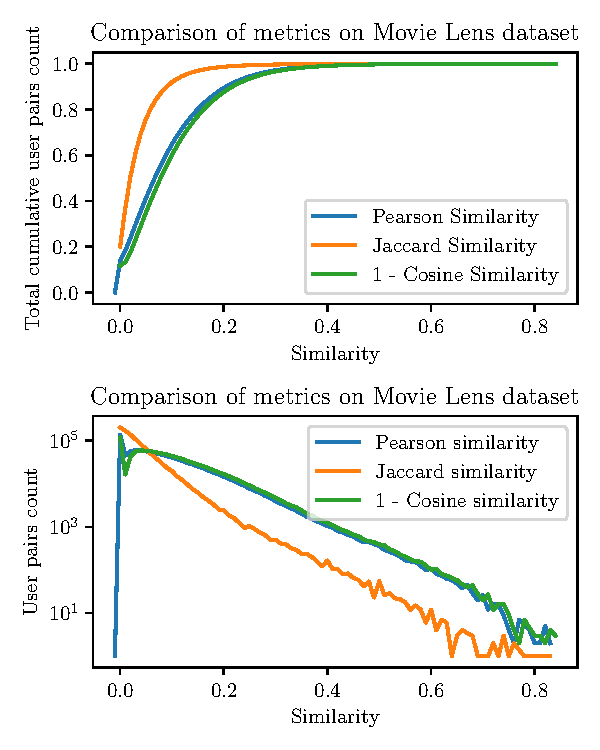
\includegraphics{img/figures/similarity_metrics.pdf}
    \caption{Comparison of similarity metrics on Movie Lens dataset.}
    \label{fig:similarity_metrics}
\end{figure}

% We have additionally considered Cosine similarity, but in our case it is important to consider only ratings that are a positive match due to most user item ratings not being present and therefore having value of '0'. The Cosine similarity would put users with sparse item ratings closer together due to taking matching 'zeros' as similar. The same hold for Jaccard similarity if we allow the intersection to match on 'zeros'.

We have compared the similarity metrics on a random sample of 1 million user pairs on \ref{fig:similarity_metrics}. Originally, we wanted to select Pearson Correlation Coefficient based on the before mentioned stability, but interestingly, PCC and the Cosine similarity are overlapping substantially. This is due to the ratings being very sparse which causes the means in PCC calculations to be close to 0 which then corresponds to the Cosine similarity. Further, PCC and Cosine similarity on average have more samples with higher similarity and less samples with lower similarity. We therefore select Cosine similarity as our similarity metric, due to its similarity to PCC and better properties than Jaccard similarity.

Now, we have a method of how to determine a similarity of two users. Further, we need to have a way of how to modulate the amount of similarity in the group. There is many interesting ways as how to create synthetic groups. Let us now present some of them.

Some of possible types of group creation:
\begin{itemize}
    \item \textbf{Random:}
        Randomly sample without replacement from the user-pool.
        
    \item \textbf{Similar:}
        Select one user randomly as a pivot, then fill in the remaining group spots with users that are as similar as possible. This basically is the k-nearest neighbours algorithm. Problem with this approach is that very rarely we encounter situations like this in the real world. Another problem is that selecting the most similar users is computationally expensive as we need to compute similarity between the pivot and every other user in the dataset. Which is not ideal for the sizes of our data.
        
    \item \textbf{Somehow similar, with outliers:}
        One other way how to relax the similarity is to randomly select a pivot user and then select the nearest neighbours only from a random subset of the whole user-pool. This way, we still get pretty similar users and do not need to perform so much computation.
        
        Other idea would be to select the next candidate based on the similarity to the last selected user instead of the pivot. In a way creating a chain of users based on the similarity of the individual links(users). This way, we could create more variable preference among the group members with still overlapping user-item interactions.
        
        Additionally, instead of selecting top-k similar users, we can make random steps in the similarity ordering, such as if we have 1000 most similar users ordered by the similarity metric, we do not need to take the top-k best ones, but for example 100th most similar, 200th most similar and so on.
        
        Further, instead of a top-k, we can select users based on a weighted probability generated either from the similarity or from the ordering of all the candidate members.
        
    \item \textbf{Similar to the whole group:}
        Instead of selecting candidates to be similar to a single main user, we can select next group members to incrementally be similar to group members already assigned, either by aggregating the ratings or by for example Borda count, this has the advantage of easier candidate selection, due to the bigger possible preference overlap. But it has a disadvantage of needing to perform more computation of similarity after each individual member selection.
        
    \item \textbf{Dissimilar:}
        Apart from finding group members based being as similar as possible, we can also try to create as dissimilar groups as possible. Here we can randomly select a first user and then select the next user which is as least similar as possible. Next, instead of selecting another user in the same way, we can calculate dissimilarity of all other uses with the joined preference of the users that are already selected to the group and again, select the most dissimilar one.
\end{itemize}


% -------------------------------------------------------------------------------------
\subsection{Selected approach}
% -------------------------------------------------------------------------------------
Let us now specify, in detail, the methods that we use and how we set the required parameters.

Easiest and most convenient option would be to calculate the similarity matrix for all users and then select groups based on this single calculation. But, this matrix can become pretty huge with the growing amount of users. Lets assume our worst case of 1,000,000 users of the Spotify dataset. Then we will have $10^{12}/2$ of similarity calculations that need to be processed and stored. This becomes difficult to manage as the amount of memory needed would be around on the order terabytes and the time needed for processing on the order of hours or days. We therefore opt for an iterative approach, where we randomly select only a smaller subset of potential group members and select the actual group members from this smaller group instead of the whole user pool. This can lead to calculating the users' similarity multiple times, but that that situation is somewhat unlikely and in total we will save orders of magnitude worth of similarity calculation (potentially depends on the number of groups we want to generate).

\subsubsection{At random}
Straightforward approach that generates groups with very distinct user preferences. We select the desired amount of users for one group from the user-pool and assign them together. Then repeat with the whole user-pool (not removing the selected members) again.

\subsubsection{Similar groups with top-k selection}
We select one user as a pivot of the group at random. Next we select some amount of users at random from the dataset as candidates and calculate the similarity between the pivot and each of the selected user candidates. Next we select the top-N most similar users to the pivot where N is the desired group size - 1 and fill in the rest of the group with these top-N most similar.

This ensures that there will be a pressure for similarity using the top-K mechanism as well as some variety due to the random selection of candidates.

\subsubsection{Similar groups with probability respecting similarity (PRS)}
We perform the same random selection as in the previous method for similar groups, but with a different procedure in the second step of selection from the candidates. We would like to select a candidate with a probability that corresponds to their similarity with the pivot user and decreases quite heavily to still ensure there is enough of a push towards selecting similar users.

\begin{figure}[ht!]
    \centering
    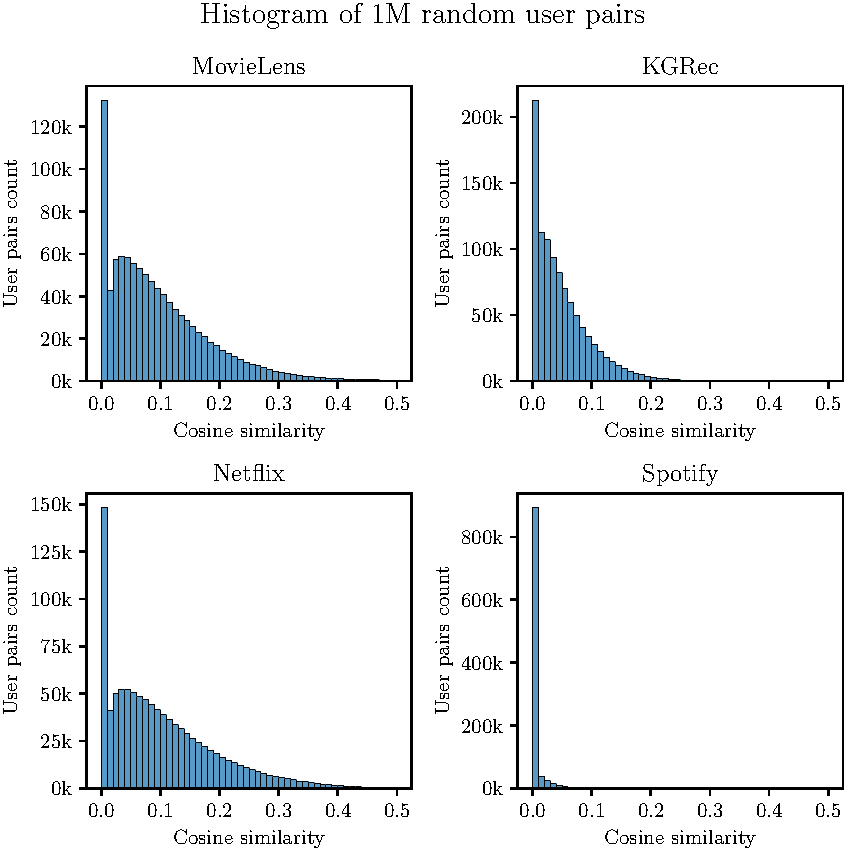
\includegraphics{img/figures/histogram_cosine_all.pdf}
    \caption{Histogram of cosine similarity of 1 million random user pairs from Movie Lens dataset.}
    \label{fig:cosine_all_histogram}
\end{figure}

Due to the exponentially decreasing number of users with higher similarity scores as can be seen on Figure \ref{fig:similarity_metrics} and in detail on Figure \ref{fig:cosine_all_histogram}, we need to ensure that potential group members with higher similarity still retain overall higher probability of being selected. We can do that by presetting the desired probability to the each cosine similarity group and then dividing this probability by the average number of user pairs in that similarity group.

Unfortunately, we do not have the precise average number of user pairs, which would require to compute similarity between all possible pairs. We can get a good estimation by sampling some amount of user pairs and calculating the ratio between the size of the group and the number of total samples. Sample of size 1 million on all datasets can be seen on Figure \ref{fig:cosine_all_histogram}.


In order to avoid deciding on the correct amount of bins to split the data into and how to smooth and sample from the bins, we have selected to model the expected cosine similarity probability density function minimizing the L2 norm. That allows us then to calculate what is the expected amount of samples in a small neighbourhood. For Movie Lens have selected an exponential distribution with parameter $\lambda=0.08918$. This distribution models our underlying data quite well, comparison can be found in Table \ref{table:5.3_modeled_comparison}. Most important portion of samples between 0.4 to 0.8 where most of the members with highest chance of being selected will fall, seems to be modeled quite precisely.
Then we can express the average expected amount of similarity pairs with similarity of $x$ in some small constant sized neighbourhood of size $NS$ to be:
\begin{equation}
    expectedSampleRatioOnInterval(x, N, \lambda) = cdf(exp(\lambda), x + N) - cdf(exp(\lambda), x),
\end{equation}
where cdf stands for the cumulative distribution function of in this case exponential distribution with the $\lambda$ parameter of $0.08918$.

\begin{table}[!ht]
    \centering
    \begin{tabular}{ c | c | c}
       cosine sim. & sampled data & $exp(\lambda=0.08918)$ \\
        \hline
        $\left[ 0.0, 0.1\right)$ & 600,716 & 674,139 \\
        $\left[ 0.1, 0.2\right)$ & 275,099 & 219,675 \\
        $\left[ 0.2, 0.3\right)$ & 90,355 & 71,583 \\
        $\left[ 0.3, 0.4\right)$ & 24,265 & 23,326 \\
        $\left[ 0.4, 0.5\right)$ & 6,660 & 7,601 \\
        $\left[ 0.5, 0.6\right)$ & 2,181 & 2,476 \\
        $\left[ 0.6, 0.7\right)$ & 602 & 807 \\
        $\left[ 0.7, 0.8\right)$ & 110 & 263 \\
        $\left[ 0.8, 0.9\right)$ & 12 & 85 \\
        $\left[ 0.9, 1.0\right]$ & 0 & 27 \\d
        total & 1,000,000 & 999,982
            
    \end{tabular}
    % \caption[Rating of selected GRS datasets.]{Rating of selected GRS datasets. Note for 'n/a' - we were unable to download the dataset, therefore unable to asses this criteria}
    \caption{Comparison of histograms of data sampled from the dataset and the created data model.}
    \label{table:5.3_modeled_comparison}
\end{table}

But we are not necessarily interested in the expected amount of samples on an interval, the main requirement is to have a ratio of expected occurrence between the sampled similarities. We are uninterested in the actual value, therefore approach using a probability density function of the modeled distribution is better. We can calculate the ration as follows:

\begin{equation}
    expectedSampleRatio(x, \lambda) = pdf(exp(\lambda), x) = \lambda e ^{-\lambda x},
\end{equation}
where pdf represents the probability density function.

Next, we need to have a way as how to scale the actual similarity. We would like to have a non-linear difference between samples. If a sample $A$ has similarity higher than sample $B$ by $0.1$, then we would like to have the sample $A$ to be selected twice as likely. Further, we can generalize the the difference as parameter $D$ and the multiplying factor as $M$.

We get:
\begin{equation}
    scale(x, D, M) = M^{\frac{1}{D}x} = M^{\frac{x}{D}},
\end{equation}
where for doubling the probability every 0.1 similarity difference will become:

\begin{equation}
    scale(x, 2, 0.1) = 2^{\frac{x}{0.1}} = 2^{10x}.
\end{equation}


\begin{equation}\label{eq:weight}
    \begin{aligned}
        weight(x, D, M, \lambda) &= \frac{scale(x, D, M)}{expectedSampleRatio(x, \lambda)} \\
        & = \frac{M^{\frac{x}{D}}}{\lambda e ^{-\lambda x}}
    \end{aligned}
\end{equation}

The parameter D in scale calculation has a big impact on the scaling, and unfortunately it needs to be tuned to each dataset separately due to the different ratings distributions as can be seen on Figure \ref{fig:cosine_all_histogram}. Through experimentation we have observed that the value of 0.1 seems to give us good results on every dataset apart for Spotify, where the width needs to be shortened substantially. We solve this situation by setting the parameter to the width of the interquartile range of the sampled ratings. In other words, we set it to the width of the middle 50\% mass for each dataset. We can see the resulting parameters for each dataset based on 1 million random user pairs in Table \ref{table:5.3_interquartile_width}. 

\begin{table}[!ht]
    \centering
    \begin{tabular}{ l l}
        dataset & \makecell[l]{interquartile \\ width (D)} \\
        \hline
        MovieLens & 0.104 \\
        KGRec & 0.057 \\
        Netflix & 0.114 \\
        Spotify & 0.025
            
    \end{tabular}
    % \caption[Rating of selected GRS datasets.]{Rating of selected GRS datasets. Note for 'n/a' - we were unable to download the dataset, therefore unable to asses this criteria}
    \caption{Scaling width parameter based on interquartile range of each dataset.}
    \label{table:5.3_interquartile_width}
\end{table}



\begin{algorithm}
	\caption{Generate groups with probability respecting similarity}
	\begin{algorithmic}[1]
	    \State Select scaling parameter $M$ and the desired amount of samples $S$ and amount of candidates $C$
	
	    \vspace{3mm}
	
	    \For {Desired number of samples $S$}
    	    \State Select random pair for users $u1$ and $u2$ from the user-pool
    	    \State Calculate similarity of $u1$ and $u2$ and store it
	    \EndFor
	    \State Fit an exponential distribution to the stored values
	    \State Calculate the width between 25th and 75th quartile as parameter D
	    \State Get its parameter $\lambda$
	    
	    \vspace{3mm}
	    
	    \For {Number of desired groups}
    	    \State Select 1 user $uCaptain$ from the user-pool as main user
    	    \State Select $C$ random users as $uCandidates$ from the user-pool
    	    \For {Each user $u$ from $uCandidates$}
    	        \State Calculate similarity between $uCaptain$ and $u$ as $sim$
    	        \State Calculate random candidate weight with (Eq. 5.8):
    	        \State $weight$ = scale($sim$, D, M) / expectedSampleRatio($sim$, $\lambda$)
    	    \EndFor
    	    \For{ Desired group size - 1}
    	    \State Perform weighted random selection on the candidates using the weights
    	    \State Add the selected user to the group and remove it from the candidates
    	    \EndFor
        \EndFor
	\end{algorithmic}
	\label{alg:create_sim_groups}
\end{algorithm} 



This gives us a framework as how to assign each candidate member a weight by which we can perform a weighted random choice and therefore introduce more variability into the group selection process. The full equation for a sample's weight can be calculated with equation \ref{eq:weight}, further, we describe the whole group generation process in Algorithm \ref{alg:create_sim_groups}.










% Pearson Correlation Coefficient due to its stable performance as mentioned in \cite{similarity_measures_comparason},  and due to its wide use among the recommender system domain.

% \textbf{Pearson correlation coefficient} for two vectors $X$ and $Y$ can be computed as follows:
% \begin{equation}
%     P(X,Y) = \frac{\text{cov}(X,Y)}{\sigma_x \sigma_y}
%     = \frac{{}\sum_{i=1}^{n} (x_i - \overline{x})(y_i - \overline{y})}{\sqrt{\sum_{i=1}^{n} (x_i - \overline{x})^2(y_i - \overline{y})^2}},
% \end{equation}
% where $cov$ is the covariance, and $\sigma$ is the standard deviation.

% Further we have selected \textbf{Jaccard similarity} due to its simplicity:
% \begin{equation}
%     J(X,Y) = \frac{|X \cap Y|}{|X \cup Y|} = \frac{|X \cap Y|}{|X| + |Y| - |X \cap Y|}.
% \end{equation}
% It has a 

% -------------------------------------------------------------------------------------
\subsection{Evaluation of the generated groups}
% -------------------------------------------------------------------------------------

% TODO: We want to evaluate the selected methods
% first, select how to measure,
% present our measurement graficek

We have implemented and used the selected techniques to generate synthetic groups. Let us now evaluate the performance of each method. And discuss the parameters of the generation process.

The random method is the simplest from the point of selecting parameters of the group creation. It does not have any.

Next, the top-k method, it only has a single parameter of the number of candidates from which we choose the actual group members. We have set the default number of candidates to 1000, due to the computational complexity rising linearly with the amount of candidates.

And lastly, the our PRS method. It has 3 parameters in total, where $\lambda$ is parameter of the exponential distribution fitted to a sample of user similarities. D is the distance and M the multiplier factor of the scale ratio. We have set the distance to be 0.1 and we vary the multiplier factor from 0,5 to 4.

We aim to compare the mean inter-group similarity. First, we define subset of size $n$ of set $S$ as

\begin{equation}
    R(S, n) := { x \in \mathcal{P}(S) : |x| = n},
    \end{equation}
where $\mathcal{P}$ is a powerset, set of all subsets. 

Then we define the inter-group similarity which represents the mean of similarity between all tuples in the group as
\begin{equation}
    intergroupSimilarity(G) = \frac{1}{|R(G,2)|}\mathlarger{\sum}_{\{a,b\} \in R(G,2)}  cos(a,b).
\end{equation}


\begin{figure}[ht!]
    \centering
    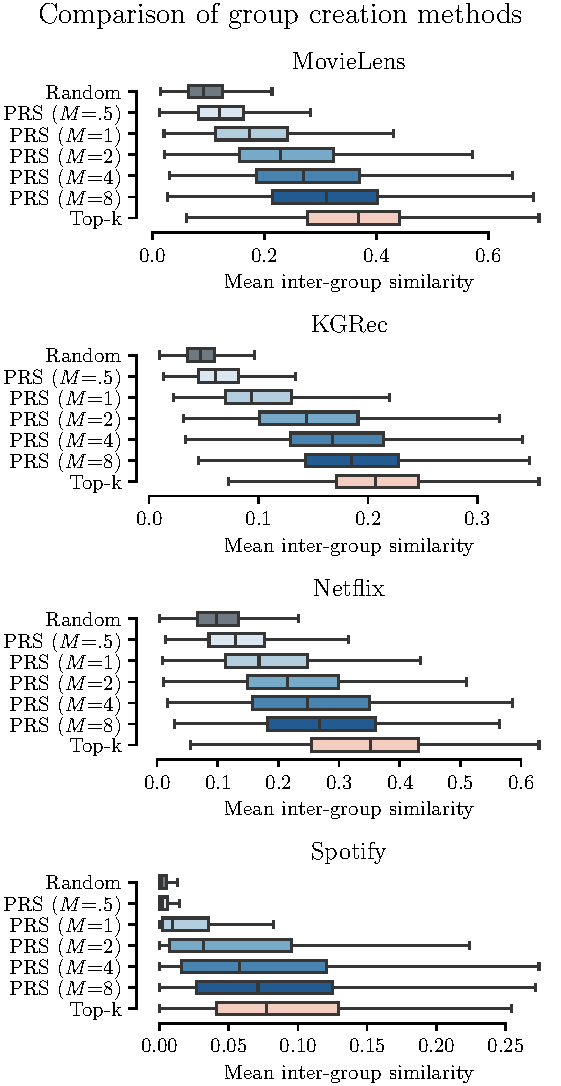
\includegraphics{img/figures/inter_group_means.pdf}
    \caption[Comparison of Random, Top-k and multiple variants of PRS group generation of size 5.]{Comparison of Random, Top-k and multiple variants of PRS group generation for groups of size 5. Number of candidates for PRS and Top-k was 1000.}
    \label{fig:inter_group_means}
\end{figure}

With each group generation method we have created 1000 groups of size 5. The resulting mean inter-group similarities can be seen on Figure \ref{fig:inter_group_means}. As expected, the random and top-k have the least and most mean inter-group similarity. With PRS we have achieved the desired scaling of the mean inter-group similarity between the random and top-k. Further more, we see that PRS generates groups that are comparably or more varied in the similarity as top-k, this is important. Other methods, which manage to create groups that utilize some sort of similarity scaling such as in \cite{GFAR-kaya2020} that select candidates based on their similarity with the pivot will not produce groups that vary in the inter-group similarity.

At first PRS did not scale well on the Spotify dataset with parameter D set to 0.1. The dataset has its similarity concentrated closer to zero. The reason for this is that most users (playlists) did rate not more than 30 items. Majority ratings are between $0$ and $0.1$, we therefore need to set the scaling width to a lower value in order to compensate for this. Based on this we have introduced the technique of setting the D parameter to the width of the interquartile range which solves the issue and decreases the amount of parameters that need to be tuned to only one - the scaling parameter M. 

In conclusion, we are satisfied with the PRS technique. It provides us with a method how reliably generate groups of varying inter-group similarity which are more heterogenous and therefore closer to reality than selecting group members directly based on the desired similarity.

\section{Dataset tool} \label{sec:dataset_tool}

We have created a Python CLI tool that allows users to download and process datasets mentioned in \ref{sec:single_user_datasets} and create artificial groups with methods described in \ref{sec:creation_of_artificial_groups}.

\todo[inline]{add parameters, screenshot and requrements}

% - clanky co cituji gfar vytvarely umele skupiny, prozkoumat,
% - lada clanek jednotlive popisy
% - porovnani prozkoumani a nasledne shrnuti/vylepseni
